\section{Experiments}\label{sec:experiments}

The study has four parts. A simulator with known ground truth checks each guarantee against the truth (Section~\ref{sec:exp-synth}), including
the horizon-resolved delay law (Section~\ref{sec:exp-horizon}). A closed-loop stream in which a model-based planner steers the state tests the endogeneity claim
(Section~\ref{sec:exp-endo}). Replicated real-video experiments compare ATLAS with standard monitors on identical streams (Sections~\ref{sec:exp-real}--\ref{sec:exp-baselines}).
Ablations, including the cases where design choices fail, close the section (Section~\ref{sec:exp-abl}). Unless stated, $\alpha=0.05$, the bet is a mixture over 20 values, and
horizons are run on non-overlapping chains at level $\alpha/H$. Code and per-experiment JSON outputs are in the supplementary material.

\subsection{Ground-truth validation}\label{sec:exp-synth}

The environment is a stable linear-Gaussian latent system whose world model uses the pre-change parameters, so it is exactly faithful until an unmodelled force of size $f$ is added at a known round
(Appendix~\ref{app:details}). The statistic is the standardized Gaussian excess of Example~\ref{ex:gauss}.

\paragraph{No false revocation.} Over $400$ null deployments of $700$ rounds, no horizon among $\{1,2,5,10,20\}$ was ever revoked, against a per-horizon bound of $0.01$ and an any-horizon bound of $0.05$.
In the horizon-resolved study below (seven horizons, $400$ null runs of $2{,}400$ rounds) the any-horizon rate is $0.005$. The rates sit far below the bound, as expected for an e-process that is a supermartingale under the null.

\paragraph{Detection delay.} Sweeping the drift margin over $100$ seeds, the measured delay matches $(\log(1/\alpha)+\log m)/D^\star$ to within about $6\%$, with $\text{delay}\cdot D^\star\approx6$, and scales as $1/D^\star$ (Figure~\ref{fig:validity}).
In this range the bet saturates, $D^\star\propto$ margin, and delay scales as one over the margin; the $1/\text{margin}^2$ regime of Theorem~\ref{thm:delay} requires margins below about $0.07$.

\begin{figure}[t]\centering
\begin{subfigure}{0.49\textwidth}\centering
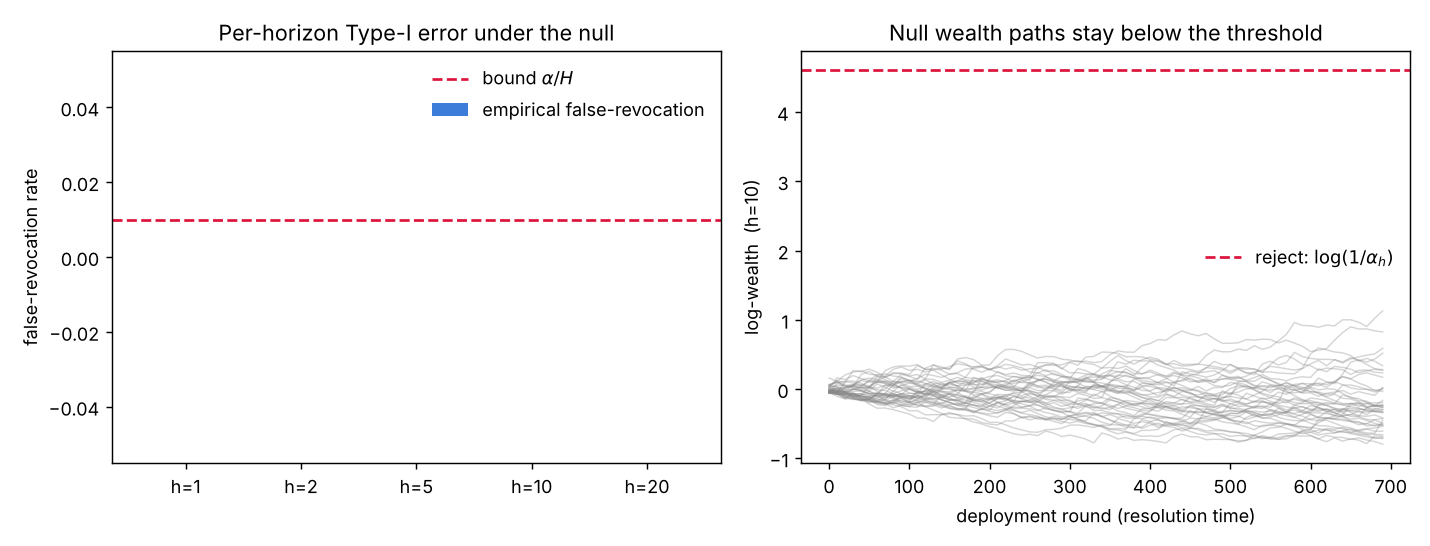
\includegraphics[width=\textwidth]{figures/exp1_validity.png}
\caption{Per-horizon false revocation under the null (left) and null wealth paths (right).}
\end{subfigure}\hfill
\begin{subfigure}{0.49\textwidth}\centering
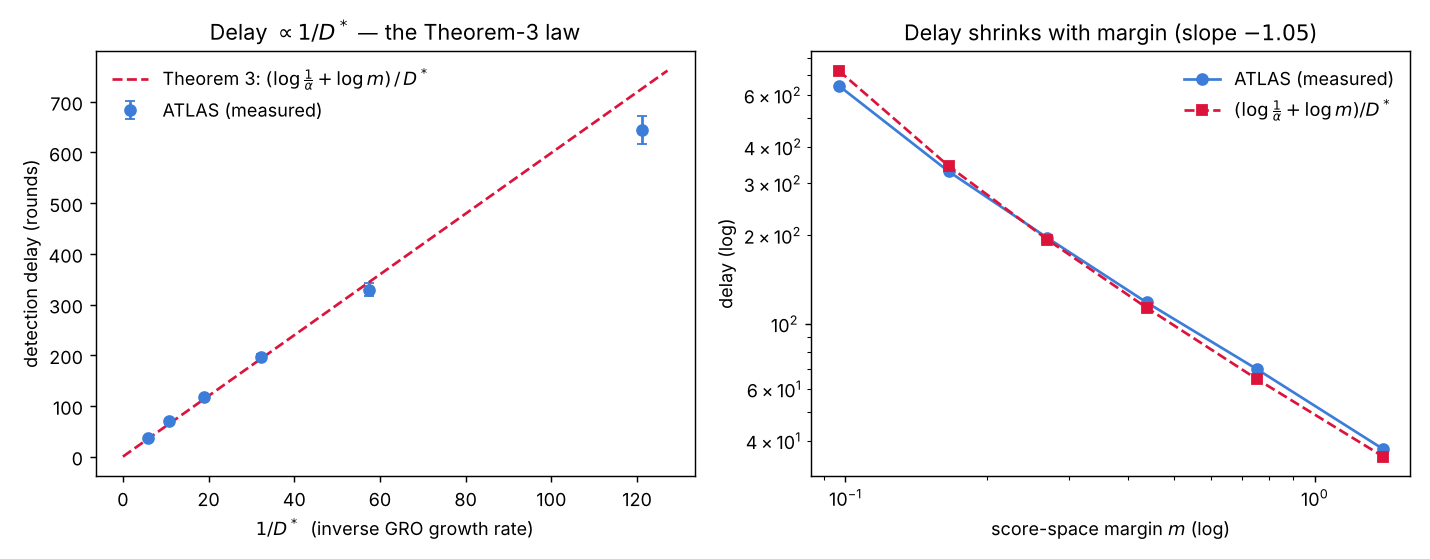
\includegraphics[width=\textwidth]{figures/exp3_delay.png}
\caption{Delay against the predicted $(\log\frac1\alpha+\log m)/D^\star$ (left) and against $1/D^\star$ (right).}
\end{subfigure}
\caption{Ground-truth validation of Theorems~\ref{thm:validity} and \ref{thm:delay} on the simulator.}
\label{fig:validity}
\end{figure}

\paragraph{The frontier and the certified gap.} With a drift of size $0.6$ opening at round $900$ (Figure~\ref{fig:teaser}), horizons $1,2,3,5,8,12,20$ are revoked $85,120,84,105,132,144,220$ rounds
after the change; the frontier falls from $20$ to $0$, first dropping $84$ rounds after the change, while an offline estimate frozen at deployment stays at $20$. The windowed certified gap
is never below the true window-average gap. It is also loose: $1.63$ nats before the change when the true gap is zero and $3.67$ after against a true $1.80$. A certificate is not a point estimate; it costs data (Section~\ref{sec:discussion}).

\begin{figure}[t]\centering
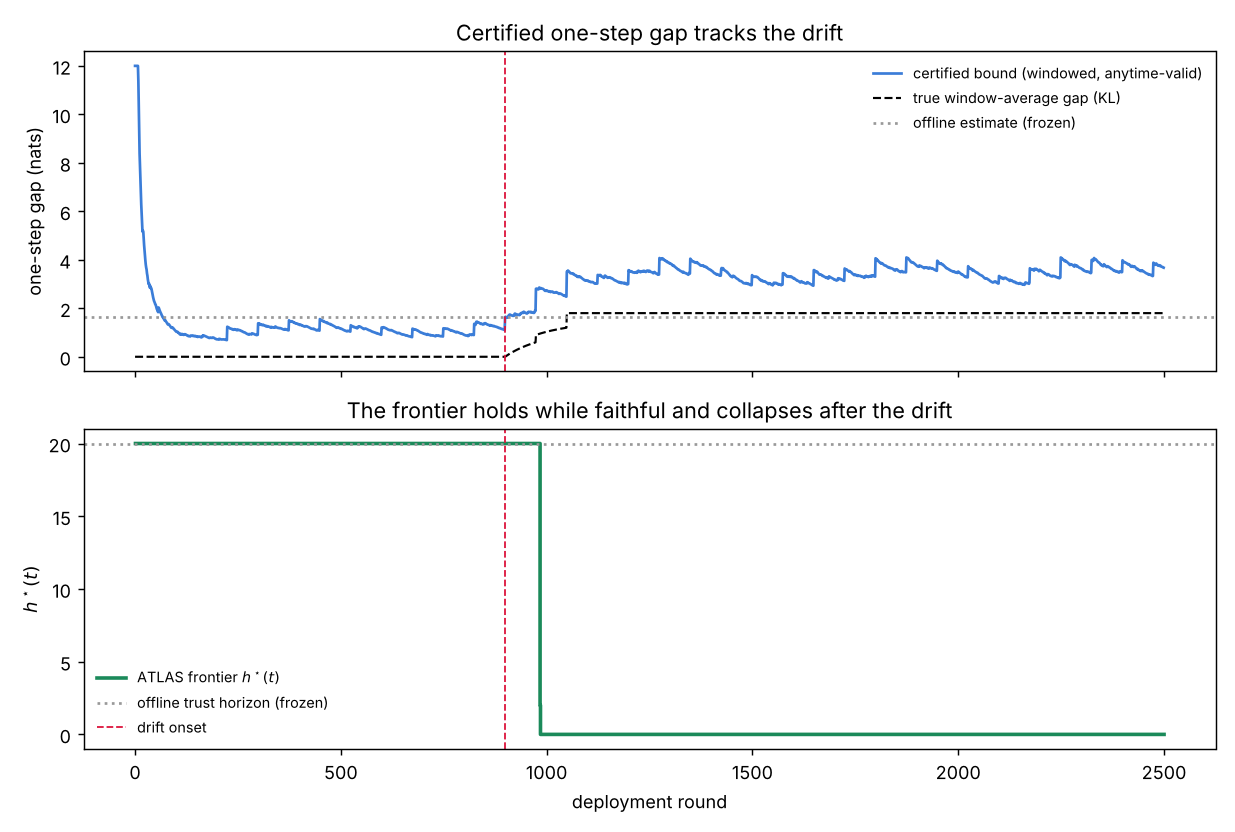
\includegraphics[width=0.78\textwidth]{figures/exp2_frontier.png}
\caption{A dynamics drift opens at round $900$. Top: the windowed, anytime-valid bound on the one-step gap (solid) against the true window-average gap (dashed) and a frozen offline estimate (dotted). Bottom: the revocation frontier $\hstar(t)$.}
\label{fig:teaser}
\end{figure}

\paragraph{The certified horizon.} Using one chain per horizon with windows of $400$ rounds, the certified total-variation bound of Theorem~\ref{thm:cert} was checked against the closed-form truth over $150$ deployments, at checkpoints
before the drift and $300$, $800$ and about $2{,}000$ rounds after it, for $h\in\{1,3,8\}$ (Table~\ref{tab:cert}). It was never violated ($0/150$ at every cell; the guarantee allows $5\%$) and its slack, bound over truth, is between $1.6$ and $3.0$ after the change. The slack at
$h=1$ is largest because Pinsker's inequality is loose for a mean shift.

\begin{table}[t]\centering
\caption{Certified total-variation bound against the exact value, $150$ deployments, drift size $0.25$ opening at round $500$. Violations: $0$ in every cell. Median slack = bound / truth.}
\label{tab:cert}
\small
\begin{tabular}{@{}lcccc@{}}
\toprule
 & true TV$_h$ & slack $+300$ & slack $+800$ & slack $+\sim2000$ \\
\midrule
$h=1$ & $0.307$ & $2.83$ & $2.17$ & $2.29$ \\
$h=3$ & $0.456$ & $2.96$ & $2.19$ & $2.19$ \\
$h=8$ & $0.635$ & $2.13$ & $1.58$ & $1.58$ \\
\bottomrule
\end{tabular}
\end{table}

\subsection{Horizon-resolved delay and the pooling negative result}\label{sec:exp-horizon}

Theorem~\ref{thm:delay}(c) predicts that horizon $h$ pays a factor $h$ for fewer updates and gains through a larger margin as the drift compounds. We measure the rounds from the change to revocation for each horizon
($150$ runs, drift $0.25$) and compare with $h(\log(H/\alpha)+\log m)/D^\star_h$, where $D^\star_h=\sup_\lambda\E\log(1+\lambda Z)$ is estimated by Monte Carlo from the post-change stationary statistic (Table~\ref{tab:horizon}, Figure~\ref{fig:horizon}).

\begin{table}[t]\centering
\caption{Rounds from the drift to revocation, by horizon. Prediction uses only the post-change statistic law. The interleaved estimator takes the first crossing over all $h$ offset chains at the threshold raised by $\log h$.}
\label{tab:horizon}
\small
\begin{tabular}{@{}lccccccc@{}}
\toprule
horizon $h$ & 1 & 2 & 3 & 5 & 8 & 12 & 20 \\
\midrule
growth rate $D^\star_h$ & $0.016$ & $0.031$ & $0.044$ & $0.067$ & $0.100$ & $0.136$ & $0.186$ \\
predicted delay & 502 & 521 & 543 & 594 & 635 & 699 & 852 \\
measured, single chain & 507 & 484 & 497 & 523 & 537 & 585 & 732 \\
measured, interleaved & 507 & 476 & 494 & 554 & 617 & 712 & 923 \\
\bottomrule
\end{tabular}
\end{table}

\begin{figure}[t]\centering
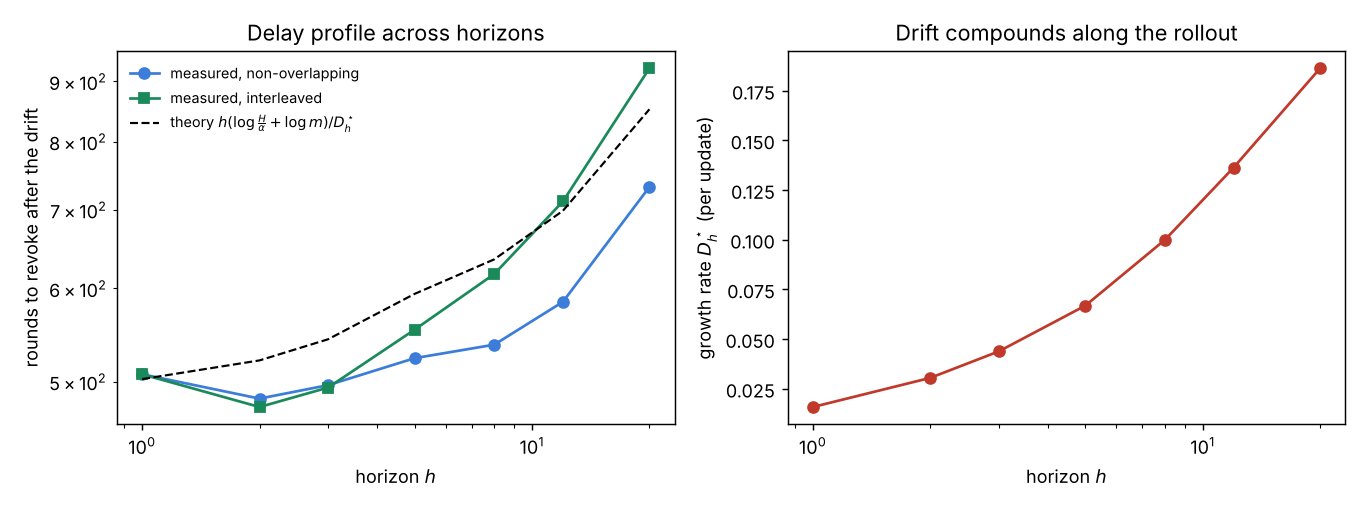
\includegraphics[width=0.86\textwidth]{figures/exp5_horizon_delay.png}
\caption{Left: measured delay (single chain and interleaved) against the prediction. Right: the growth rate $D^\star_h$ rises with the horizon because the drift accumulates along the rollout.}
\label{fig:horizon}
\end{figure}

The prediction is within $16\%$ of the measurement at every horizon and errs on the conservative side. Two features are worth stating plainly. First, in this system $D^\star_h$ grows roughly in proportion to $h$, so the factor-$h$ loss
is almost exactly offset and delay in rounds is nearly flat in $h$ (between $484$ and $732$); long horizons are not slower \emph{here}, but nothing in the theory says that must hold for other dynamics. Second, the interleaved estimator,
which was meant to win back the data discarded by non-overlap, is no faster and is slower at long horizons ($923$ against $732$ rounds at $h=20$), as the pooling argument of Section~\ref{sec:overlap} predicts. Under the null both
estimators stay valid (any-horizon false revocation $0.005$ and $0.003$).

\subsection{Policy-endogenous streams}\label{sec:exp-endo}

We test the claim that exchangeability- and calibration-based monitors lose validity when the planner steers the state, on a closed-loop latent world model with state-dependent noise in which the world model is
exactly faithful, so every alarm under the null is a false alarm (Appendix~\ref{app:details}). Four planners generate the stream: exogenous exploration (\emph{exo}); a certainty-equivalent controller run through the model toward a low-noise state (\emph{low}) or
toward a high-noise state (\emph{high}); and a monitor-aware planner (\emph{adv}) that runs ATLAS's own e-process on the stream it produces and moves to the high-noise region whenever the wealth is positive. The mean noise level induced is $0.24$, $0.15$, $0.33$ and $0.15$ respectively.
Each monitor sees either the \emph{raw} squared prediction error, the quantity practitioners monitor, or the model-\emph{standardized} statistic that ATLAS uses. Tunable detectors are calibrated to a $5\%$ false-alarm rate at $400$ rounds on a separate exogenous calibration deployment, the
usual offline protocol, then run for $1{,}200$ rounds under each planner ($300$ runs each).

\begin{table}[t]\centering
\caption{False-alarm rate on a closed-loop stream with a faithful model: at $400$ rounds / by $1{,}200$ rounds, $300$ runs per cell. Tunable detectors are calibrated on exogenous data to $5\%$ at $400$ rounds. ``raw'' monitors see squared prediction error, ``std'' monitors the standardized statistic.}
\label{tab:endo}
\small
\setlength{\tabcolsep}{4pt}
\begin{tabular}{@{}llcccc@{}}
\toprule
stream & monitor & exo & low & high & adv \\
\midrule
raw & CUSUM            & .07/.22 & .00/.00 & \textbf{1.00/1.00} & .40/.49 \\
raw & Page--Hinkley    & .04/.38 & .00/.00 & .01/.13 & .45/.73 \\
raw & ADWIN            & .12/.53 & .00/.04 & .00/.01 & .54/.73 \\
raw & KSWIN            & .06/.18 & .00/.06 & .00/.01 & .20/.40 \\
raw & Conformal MG     & .09/.10 & .00/.00 & \textbf{1.00/1.00} & .44/.49 \\
\midrule
std & CUSUM            & .09/.28 & .07/.23 & .09/.25 & .08/.26 \\
std & Page--Hinkley    & .08/.56 & .08/.54 & .06/.56 & .07/.52 \\
std & ADWIN            & .03/.19 & .05/.20 & .05/.16 & .04/.17 \\
std & KSWIN            & .02/.08 & .03/.08 & .03/.06 & .02/.08 \\
std & Conformal MG     & .03/.03 & .03/.03 & .01/.01 & .02/.02 \\
\midrule
std & \textbf{ATLAS}   & \textbf{.00/.01} & \textbf{.00/.01} & \textbf{.00/.01} & \textbf{.00/.01} \\
\bottomrule
\end{tabular}
\end{table}

Three patterns appear in Table~\ref{tab:endo}. (i) Calibrated offline on exogenous data, raw-error monitors do not carry over: CUSUM and the conformal martingale alarm in every run when the planner heads for the
high-noise region, and under the monitor-aware planner every raw monitor reaches $0.40$--$0.73$; under the low-noise planner the same monitors alarm almost never, which would mask a real drift. (ii) On the
standardized stream the exchangeability-based conformal martingale is valid for \emph{every} planner. That is not an accident: when the model is exactly faithful the standardized statistic is pivotal, identically distributed whatever the planner does, so the planner cannot hurt a monitor that
sees it. The change detectors on that stream still inflate with monitoring time (Page--Hinkley $0.08\to0.56$). The honest summary is that conformal monitors are fine on a pivotal statistic and ATLAS's advantage is that it needs no
pivotality and no tuning, only a conditional-mean bound. (iii) ATLAS never exceeded $0.013$ under any planner, including the one that watches its wealth.

\paragraph{Power depends on the planner.} After an unmodelled drift of size $0.4$ at round $400$, ATLAS detected the drift in every run with mean delay $346$, $211$, $532$ and $471$ rounds under \emph{exo}, \emph{low}, \emph{high} and \emph{adv}. The planner that seeks high-noise states shields the drift
by roughly $1.5\times$ against exogenous exploration, since the same mean shift moves the standardized statistic less where the noise is larger. The conformal martingale on the standardized stream is slower by $1.6$--$2.2\times$ in every setting and misses the drift in $3$--$5\%$ of runs. Validity under endogeneity is a theorem; power under endogeneity is an empirical quantity that this study
measures for one family of planners and does not bound in general.

\begin{figure}[t]\centering
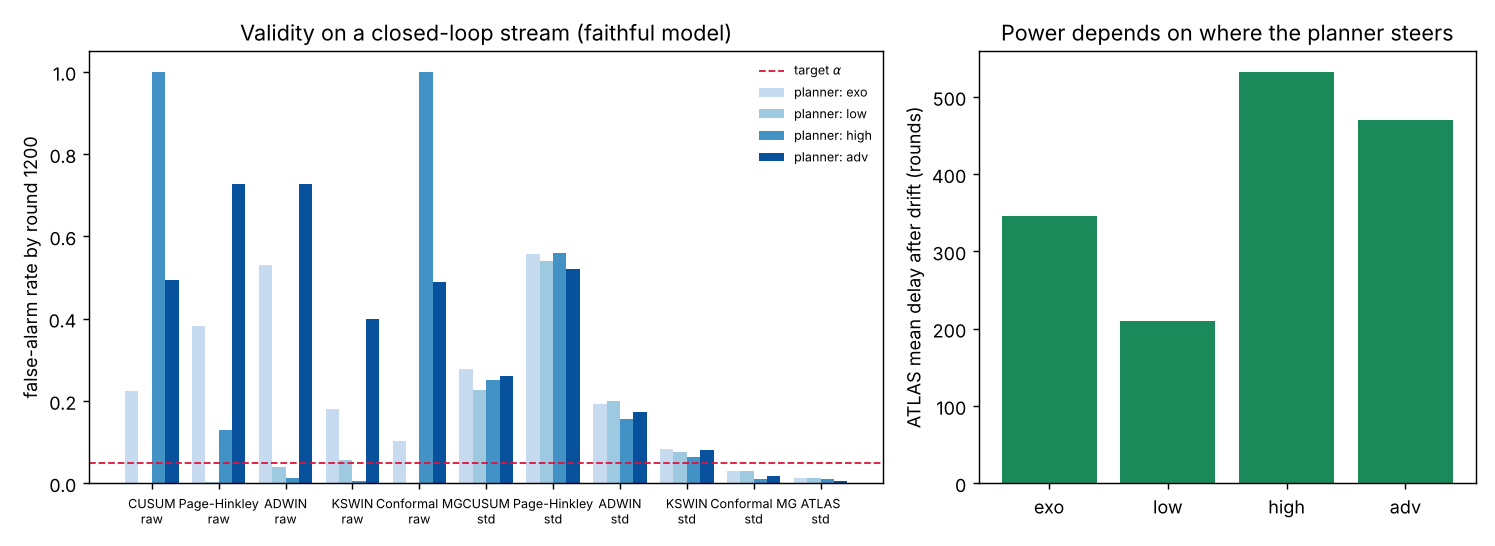
\includegraphics[width=0.9\textwidth]{figures/exp6_endogeneity.png}
\caption{Left: false-alarm rate by round $1{,}200$ for each monitor and planner on the closed-loop stream. Right: ATLAS's mean detection delay after a drift under each planner.}
\label{fig:endo}
\end{figure}

\subsection{Real video: replicated protocol}\label{sec:exp-real}

Three real shifts are studied with a PCA-plus-linear-dynamics latent world model: Moving MNIST \citep{srivastava2015movingmnist} native speed to double speed, KTH \citep{schuldt2004kth} walking to running, and KTH walking outdoors to indoors. Each
of 30 repetitions draws a fresh random split into training, calibration, in-distribution deployment and shifted deployment clips, refits the world model, and sets the tolerance $\eps_h=\bar z_h+k\,s_h$ from the calibration clips (mean $\bar z_h$ and standard deviation $s_h$ of the clipped statistic, with $k\in\{0,0.25,0.5,1\}$).
Competing detectors are tuned on a separate set of 30 repetitions to a $5\%$ false-alarm rate over the in-distribution deployment length $L$. We report false alarms over $L$ clips and over $3L$ (in-distribution clips resampled with replacement, standing in for longer monitoring), and detection rate and delay in clips after the shift, with bootstrap $95\%$ intervals.

\begin{table}[t]\centering
\caption{Replicated real-video study (30 random splits per shift). False alarms over $L$ in-distribution clips and over $3L$; detection rate and delay in clips after the shift; bootstrap 95\% intervals in brackets. $k$ is the tolerance margin in standard deviations of the calibration statistic. Tunable detectors are tuned to 5\% on separate repetitions.}
\label{tab:real}
\small
\setlength{\tabcolsep}{3pt}
\begin{tabular}{@{}lcccc@{}}
\toprule
 & FA @ $L$ & FA @ $3L$ & detection rate & delay (clips) \\
\midrule
\multicolumn{5}{@{}l}{\emph{Moving MNIST: native $\to$ double speed}} \\
ATLAS, $k=0$ & 0.17 [0.03,0.30] & 0.43 [0.27,0.60] & 1.00 & 4.3 [3.8,4.8] \\
ATLAS, $k=0.25$ & 0.00 [0.00,0.00] & 0.00 [0.00,0.00] & 1.00 & 4.6 [4.1,5.1] \\
ATLAS, $k=0.5$ & 0.00 [0.00,0.00] & 0.00 [0.00,0.00] & 1.00 & 5.2 [4.6,5.8] \\
ATLAS, $k=1$ & 0.00 [0.00,0.00] & 0.00 [0.00,0.00] & 1.00 & 6.6 [5.8,7.5] \\
CUSUM & 0.07 [0.00,0.17] & 0.43 [0.27,0.60] & 1.00 & 3.2 [2.7,3.7] \\
ADWIN & 0.07 [0.00,0.17] & 0.37 [0.20,0.53] & 0.00 & --- \\
KSWIN & 0.03 [0.00,0.10] & 0.27 [0.13,0.43] & 0.00 & --- \\
Conformal martingale & 0.53 [0.37,0.70] & 0.67 [0.50,0.83] & 1.00 & 0.3 [0.1,0.5] \\
\midrule
\multicolumn{5}{@{}l}{\emph{KTH: walking $\to$ running}} \\
ATLAS, $k=0$ & 0.43 [0.27,0.60] & 0.47 [0.30,0.63] & 1.00 & 0.3 [0.1,0.5] \\
ATLAS, $k=0.25$ & 0.17 [0.03,0.30] & 0.37 [0.20,0.53] & 1.00 & 0.5 [0.2,0.9] \\
ATLAS, $k=0.5$ & 0.07 [0.00,0.17] & 0.13 [0.03,0.27] & 1.00 & 1.3 [0.5,2.2] \\
ATLAS, $k=1$ & 0.03 [0.00,0.10] & 0.03 [0.00,0.10] & 0.70 & 5.3 [1.7,9.7] \\
CUSUM & 0.97 [0.90,1.00] & 0.93 [0.83,1.00] & 1.00 & 0.1 [0.0,0.3] \\
ADWIN & 0.17 [0.03,0.30] & 0.43 [0.27,0.60] & 0.00 & --- \\
KSWIN & 0.00 [0.00,0.00] & 0.00 [0.00,0.00] & 0.00 & --- \\
Conformal martingale & 0.70 [0.53,0.87] & 0.63 [0.47,0.80] & 1.00 & 0.9 [0.5,1.4] \\
\midrule
\multicolumn{5}{@{}l}{\emph{KTH: outdoor $\to$ indoor walking}} \\
ATLAS, $k=0$ & 0.33 [0.17,0.50] & 0.50 [0.33,0.67] & 1.00 & 1.9 [1.0,3.1] \\
ATLAS, $k=0.25$ & 0.07 [0.00,0.17] & 0.23 [0.10,0.40] & 0.93 & 3.1 [1.6,5.2] \\
ATLAS, $k=0.5$ & 0.07 [0.00,0.17] & 0.03 [0.00,0.10] & 0.77 & 4.1 [1.7,6.8] \\
ATLAS, $k=1$ & 0.03 [0.00,0.10] & 0.03 [0.00,0.10] & 0.33 & 2.3 [0.6,4.5] \\
CUSUM & 0.57 [0.40,0.73] & 0.63 [0.47,0.80] & 1.00 & 1.4 [0.9,2.0] \\
ADWIN & 0.10 [0.00,0.20] & 0.37 [0.20,0.53] & 1.00 & 6.2 [5.2,7.2] \\
KSWIN & 0.00 [0.00,0.00] & 0.00 [0.00,0.00] & 1.00 & 5.6 [4.2,7.2] \\
Conformal martingale & 0.43 [0.27,0.60] & 0.57 [0.40,0.73] & 1.00 & 0.4 [0.2,0.6] \\
\bottomrule
\end{tabular}
\end{table}


The picture is mixed, and we report it as such. With the tolerance set at the calibration mean ($k=0$), ATLAS's false-alarm rate over $3L$ clips is $0.43$ on Moving MNIST, $0.47$ on KTH walking$\to$running, and
$0.50$ on KTH outdoor$\to$indoor, all above $\alpha$: pooled-mean calibration does not satisfy the conditional null (Section~\ref{sec:exp-abl}, ablation D). Adding a margin repairs this at a cost in power. On Moving MNIST $k\ge0.25$ gives no false alarm in 30 repetitions
and detection in every repetition, with a delay of $4.6$--$6.6$ clips. On KTH, subject-to-subject heterogeneity makes the statistic far less stable and calibration clips are few: $k=0.5$ still gives $0.13$ false alarms over $3L$ clips for walking$\to$running, and
$k=1$ brings it to $0.03$ while detection drops to $0.70$; on the subtler outdoor$\to$indoor shift $k=0.5$ gives $0.03$ false alarms and detects in $0.77$ of repetitions. The false-alarm rates for $k\ge0.5$--$1$ are close to $\alpha$ but nothing here is
a guarantee, because the tolerance is estimated. The competing monitors fare worse on false alarms on these real streams: the conformal martingale alarms in $0.43$--$0.70$ of in-distribution repetitions over $L$ clips (exchangeability fails across the temporal and subject structure of the stream), CUSUM in $0.97$ on KTH walking$\to$running, and
ADWIN and KSWIN, tuned to $5\%$ on separate repetitions, either miss the shift entirely (Moving MNIST, KTH walking$\to$running) or detect it in $5$--$6$ clips (domain shift). Tuning a sensitivity to a target false-alarm rate on a limited number of
streams is itself unstable, which is the practical case for a method whose false-alarm control does not rely on it. We read the table as evidence that the construction is usable on real video when the tolerance is set with a margin and validated, not as evidence that false-alarm control transfers automatically.

\subsection{Comparison with competitor monitors on the simulator}\label{sec:exp-baselines}

On the ground-truth simulator we also compare ATLAS with CUSUM and Page--Hinkley \citep{page1954cusum}, ADWIN \citep{bifet2007adwin}, KSWIN \citep{raab2020kswin}, Bayesian online changepoint detection \citep{adams2007bocpd}, the e-detector \citep{shin2024edetectors}, and a conformal test martingale \citep{vovk2003testing}, all on the same one-step statistic stream, with tunable detectors calibrated to $5\%$ at $400$ rounds (Table~\ref{tab:baselines}).
The anytime-valid tests keep false alarms below $\alpha$ at three times the calibration horizon, while every tuned detector inflates (Page--Hinkley from $0.05$ to $0.53$); the tuned detectors' shorter delay comes from alarming more readily. The conformal martingale is also valid but slower ($77.9$ against $53.8$ rounds) and, as
Section~\ref{sec:exp-endo} shows, loses validity when fed non-pivotal scores on a steered stream.

\begin{table}[t]\centering
\caption{Simulator, $\alpha=0.05$: false-alarm rate at the calibration horizon $T_{\mathrm{cal}}=400$ and at $3T_{\mathrm{cal}}$, and mean detection delay (rounds). BOCPD tuned to the false-alarm target does not detect this drift.}
\label{tab:baselines}
\small
\begin{tabular}{@{}llccc@{}}
\toprule
 & monitor & FA @ $T_{\mathrm{cal}}$ & FA @ $3T_{\mathrm{cal}}$ & delay \\
\midrule
\multirow{2}{*}{anytime-valid} & \textbf{ATLAS} & $\mathbf{0.000}$ & $\mathbf{0.003}$ & $53.8$ \\
 & Conformal martingale & $0.023$ & $0.023$ & $77.9$ \\
\midrule
\multirow{6}{*}{tuned} & CUSUM & $0.113$ & $0.273$ & $12.2$ \\
 & Page--Hinkley & $0.050$ & $0.527$ & $30.4$ \\
 & ADWIN & $0.040$ & $0.140$ & $23.8$ \\
 & KSWIN & $0.040$ & $0.087$ & $33.4$ \\
 & BOCPD & $0.083$ & $0.083$ & --- \\
 & e-detector & $0.013$ & $0.197$ & $32.8$ \\
\bottomrule
\end{tabular}
\end{table}

\subsection{Ablations and negative results}\label{sec:exp-abl}

Table~\ref{tab:abl} collects five ablations at horizon one ($400$ null and $200$ alternative runs per cell; drift $0.25$ at round $500$ unless noted).

\begin{table}[t]\centering
\caption{Ablations. FA = false-revocation rate under the null (or, in B, revocation rate for a model whose true gap is $g=0.0138$); detect = fraction detected after the drift; delay in rounds.}
\label{tab:abl}
\small
\begin{tabular}{@{}llccc@{}}
\toprule
 & variant & FA & detect & delay \\
\midrule
\multirow{5}{*}{A. bet} & mixture (20 values) & .025 & 1.00 & 392 \\
 & plug-in (GRAPA) & .015 & 1.00 & 429 \\
 & fixed $\lambda=0.1\lambda_{\max}$ & .000 & .97 & 1397 \\
 & fixed $\lambda=0.5\lambda_{\max}$ & .030 & 1.00 & 401 \\
 & fixed $\lambda=\lambda_{\max}$ & .038 & .99 & 362 \\
\midrule
\multirow{5}{*}{B. tolerance} & $\eps=0$ & .125 & --- & --- \\
 & $\eps=0.5g$ & .055 & --- & --- \\
 & $\eps=g$ & .025 & --- & --- \\
 & $\eps=1.5g$ & .020 & --- & --- \\
 & $\eps=2.5g$ & .005 & --- & --- \\
\midrule
\multirow{3}{*}{C. drift shape} & step & .030 & .99 & 365 \\
 & ramp over 300 rounds & .030 & .99 & 607 \\
 & transient pulse (150 rounds) & .030 & .17 & 326 \\
\midrule
\multirow{3}{*}{D. statistic} & standardized excess & .025 & 1.00 & 392 \\
 & log-score vs.\ climatology, $\eps=-1$ & .000 & .00 & --- \\
 & log-score vs.\ climatology, $\eps=$ pooled null mean & \textbf{.253} & .00 & --- \\
\midrule
\multirow{2}{*}{E. noise tails} & Gaussian & .025 & 1.00 & 392 \\
 & Student-$t_5$ (variance-matched) & .007 & .98 & 821 \\
\bottomrule
\end{tabular}
\end{table}

The mixture is close to the best fixed bet without knowing it (A): a bet that is too small is slow and a large fixed bet is slightly faster but is the one that depends on guessing the margin.
Tolerance (B) behaves as designed: when $\eps$ is at or above the true gap the revocation rate is at most $\alpha$; when $\eps$ is below it the model really is outside tolerance and revocation grows, slowly, because the gap is tiny. A ramp (C) is detected late, and a short transient is mostly missed: a cumulative e-process is not
a detector of brief excursions, and users who care about transients should use a windowed variant.

Ablation D is the most important caution. The log-score advantage over a climatology reference has a \emph{state-dependent} conditional mean, because the reference ignores the state. Setting $\eps$ to its pooled null mean makes the null hold on average but not conditionally, and validity fails
($0.253$ false revocations against a $0.05$ guarantee). A constant $\eps$ that does hold conditionally (a conservative bound) is so large that the drift is never detected. The standardized Gaussian excess has a pivotal conditional mean and avoids the dilemma. The same issue applies to real video: the
tolerances calibrated on pooled calibration clips in Section~\ref{sec:exp-real} are only empirically safe, which is why the margin $k$ matters there. With heavy-tailed noise (E) the standardized statistic stays valid, since only the covariance enters its conditional mean, and detection is slower.
